\chapter{Probabilidad y Estadística}

\section{Probabilidad}
% Página 67 del cuaderno en papel

Los sucesos en probabilidad se escriben entre comillas y se representan con una letra mayúscula.

\begin{itemize}
    \item[m] $I =$ impar
    \item[m] $I =$ probabilidad de sacar un número impar
    \item[m] $I =$ "Probabilidad de sacar un número impar"
    \item[b] $I =$ "Sacar un número impar"
\end{itemize}

\textbf{Operaciones con conjuntos (o sucesos)}

$A\cup B = \{x\in A \vee x \in B\}$ (Unión)

$A\cap B = \{x\in A \wedge x \in B\}$ (Intersección - Probabilidad compuesta)

$A^c = \overline{A} = \{x\not\in A$ (Complementario) \textit{No se llama contrario}.

$A - B = \{x\in A \wedge x \not\in B\}$ (Diferencia)

\obs $A - B = A \cap \overline{B}$

\begin{defn}[Leyes\IS de de Morgan]
\[\overline{A\cap B} = \overline{A}\cup \overline{B}\]
\[\overline{A\cup B} = \overline{A}\cap \overline{B}\]
\end{defn}



\begin{defn}[Compatibilidad]
Sean $A,B$ dos sucesos.

Son compatibles si $A\cap B \not= \emptyset$. 
Son incompatibles si $A\cap B =\emptyset$
\end{defn}

\begin{defn}[Sistema completo de sucesos]
Sean $A_1,...,A_n$ sucesos de un cierto experimento aleatorio.
%
Se dice que forman un sistema completo de sucesos del espacio muestral $E$ cuando:

\begin{itemize}
    \item $\displaystyle\bigcup_{i=1}^n A_i = A_1\cup A_2 \cup ... \cup A_n =  E$
    \item $A_i\cap A_j = \emptyset\;\;\; \forall i,j=1...n$
\end{itemize}
\end{defn}

\begin{example}
Sea $E = \{1,2,3,4,5,6\}$. ¿Son sistemas completos de sucesos las siguientes agrupaciones?

\begin{itemize}
    \item $A_1 = \{1,2,3\}; A_2 = \{4,5\} ; A_3 = \{6\}$
    \item $A_1 = \{\text{múltiplos de 3}\} ; A_2 = \{\text{números pares}\} ; A_3 = \{1,5\}$
\end{itemize}
\end{example}


\begin{prop}Sea $A_1,...,A_n$ un sistema completo de sucesos. Entonces \[\displaystyle\sum_{i=1}^n P(A_i) = 1\]
\end{prop}


\begin{defn}[Regla de Laplace]
Si los socesos elementales de un experimento aleatorio son equiprobables, entonces, $P(A) = \frac{\text{casos favorables}}{\text{casos posibles}}$
\end{defn}
\obs ¿Y si no son equiprobables? 

\begin{defn}[Probabilidad\IS Ley de los grandes números]
Sea $A$ un suceso y $h(A)$ su frecuencia de ocurrencia relativa\footnote{El porcentaje de veces que ese suceso ocurre.} en $n$ repeticiones del experimento. Entonces \[P(A) = \lim_{n\leftrightarrow \infty}h(A)\]
\end{defn}


\begin{defn}[Probabilidad\IS Axiomática de Kolmogorov]
    Sea $p$ una función que asocia a cada suceso $A$ del espacio de sucesos $S$ un número real designado por $p(A)$.
    
    Decimos que $p$ es una probabilidad si cumple las siguientes propiedades:
    \begin{itemize}
        \item $0\leq p(A) \leq 1 \;\;\;\forall A\in S$
        \item $p(E) = 1$
        \item $A\cap B = \emptyset \implies p(A\cup B) = p(A) + p(B)$
    \end{itemize}
\end{defn}

\paragraph{Propiedades de la probabilidad:} Sea $A$ un suceso cualquiera:
\begin{itemize}
    \item $P(\overline{A}) = 1 - P(A)$
    \item $A\subset B \implies P(A) \leq P(B)$
    \item $0\leq P(A) \leq 1$
    \item $P(A\cup B) = P(A) + P(B) - P(A\cap B)$
\end{itemize}

\begin{center}
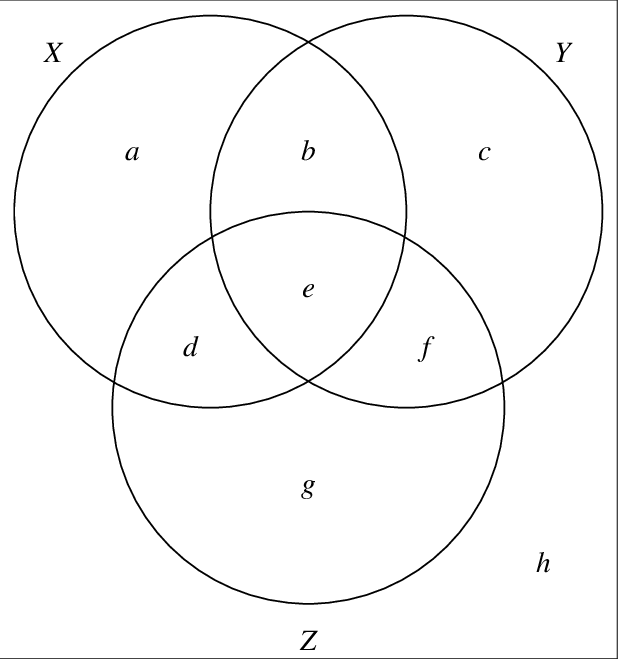
\includegraphics[scale=0.3]{img/Venn-diagram-visualization-of-a-3-event-probability-space-O.png}
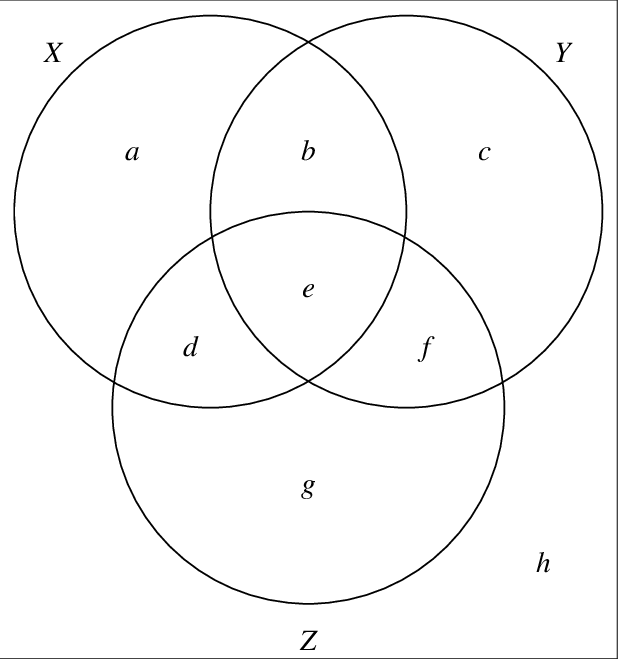
\includegraphics[scale=0.3]{img/Venn-diagram-visualization-of-a-3-event-probability-space-O.png}
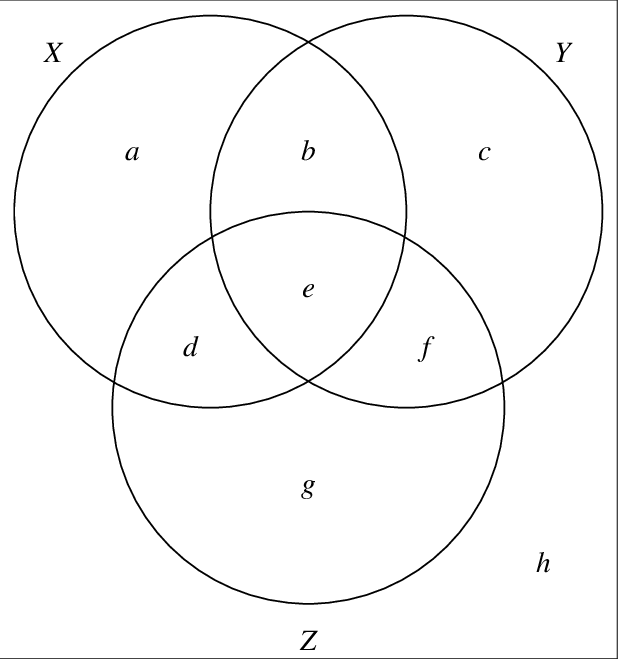
\includegraphics[scale=0.3]{img/Venn-diagram-visualization-of-a-3-event-probability-space-O.png}
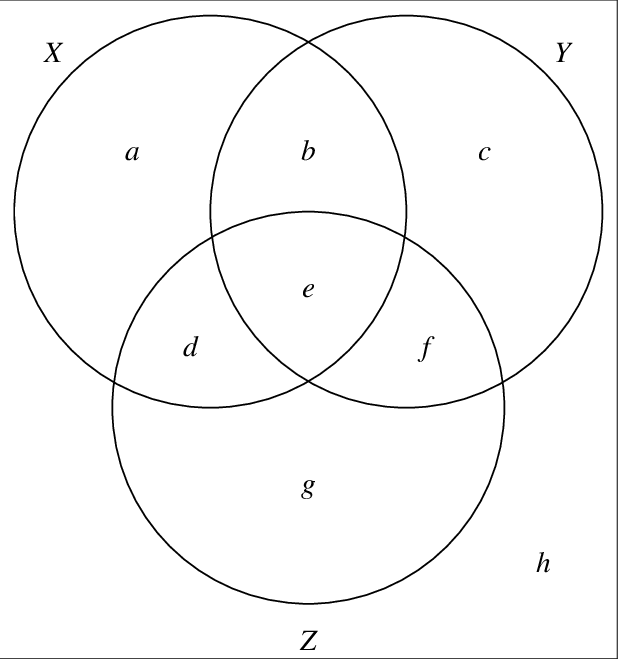
\includegraphics[scale=0.3]{img/Venn-diagram-visualization-of-a-3-event-probability-space-O.png}
\end{center}

\begin{defn}[Probabilidad\IS condicionada]
Sean $A,B$ sucesos de un suceso aleatorio. 

Se define la probabilidad condicionada $p(A/B)$ como la probablidad de que se produzca $A$ si sabemos que se ha producido $B$.

\[P(A/B) = \frac{P(A\cap B)}{P(B)}\]
\end{defn}

\textit{Este es un buen momento para hacer algún ejercicio. Página 349, ejer 36 por ejemplo. Recordamos que $P(A\cup B) = P(A) + P(B) - P(A\cap B)$}

\begin{defn}[Independencia de sucesos]
$A,B$ son sucesos independientes si y sólo si \[P(A/B) = P(A/\overline{B}) = P(A)\]
\end{defn}

\begin{theorem}
\[A,B \text{ independientes } \dimplies P(A\cap B) = P(A)·P(B)\]
\end{theorem}
\begin{proof}
\[\left.\begin{array}{c}
P(A/B) = \frac{P(A\cap B)}{P(B)} \dimplies P(A\cap B) = P(B)·P(A/B)\\A,B \text{ independientes } \dimplies P(A/B) = P(A)\end{array}\right\}*\]
\[(*) \implies P(A\cap B) = P(B)·\underset{P(A/B)}{P(A)} = P(B)·P(A)\]
\end{proof}

\begin{theorem}[Teorema\IS Probabilidad Total]
Sea $A_1,A_2,...,A_n$ un sistema completo de sucesos y sea $B$ otro suceso.
\[  
    P(B) = P(A_1\cap B) + P(A_2\cap B) + ... + P(A_n\cap B) = 
\]
\[
    P(B/A_1)·P(A_1) + P(B/A_2) · P(A_2) + ... + P(B/A_n)·P(A_n)
\]
\end{theorem}
\begin{theorem}[Teorema\IS de Bayes]
\[P(B/A) = \frac{P(A/B)·P(B)}{P(A)}\]
\end{theorem}
\begin{proof}
\[
\left.
\begin{array}{c}
    P(A\cap B) = P(A)·P(B/A)\\
    P(A\cap B) = P(B)·P(A/B)
\end{array}\right\} \implies P(A)·P(B/A) =  P(B)·P(A/B) \dimplies \]\[\dimplies P(B/A) = \frac{P(A/B)·P(B)}{P(A)} 
\]
\end{proof}


\paragraph{Bayesian trap (obtenido de youtube.com/Veritasium)}

\begin{example}
Se sabe que una enfermedad rara sólo afecta al 1\% de la población. 
%
El porcentaje de falsos positivos de las pruebas médicas es del 10\%, y el porcentaje de falsos negativos es del 1\%.

Intuitivamente, ¿cuál dirías que es la probabilida de tener la enfermedad sabiendo que has dado positivo en el test? ¿Podrías calcularlo numéricamente?

Los datos son: $P(E) = 0.01$, $P(-|E) = 0.01$ y $P(+|\overline{E})=0.1$

Aplicando el teorema de Bayes:

\[P(E|+) = \frac{P(+|E)·P(E)}{P(+)} = \frac{P(+|E)·P(E)}{P(+|E)·P(E) + P(+|\overline{E})·P(\overline{E})}= 0.01 \]
\end{example}

\section{Distribuciones de probabilidad}

Introducimos el tema con 4 preguntas que iremos contestando a lo largo del tema. Acabaremos el tema cuando sepamos contestar a las 4 preguntas.

¿Probabilidad de sacar 2 caras en 4 lanzamientos? Lo resolvemos como un árbol.

¿Probabilidad de sacar 2 caras en 10 lanzamientos? Binomial. Contestamos esta pregunta y deducimos la fórmula de la binomial. Algunos ejemplos más para interiorizar la intuición de la binomial.



Dada la fómrula, desde el libro, vamos viendo las definiciones de probabilidad. Esperanza(media) y varianza: ¿cuántas caras podemos esperar en 10 lanzamientos? Si el experimento de tirar 10 monedas lo hago 10000 veces, podría hacer la media. 

¡Unión de la probabilidad y de la estadística! Hago cosas de estadística (varianza, esperanza-media) con probabilidades.

2 ejercicios de cálculo de binomial para entender la fórmula. Después hablaremos más a fondo de la teoría de distribuciones de probabilidad.

¿Probabilidad de sacar exactamente 120 caras en 2000 lanzamientos? Casi 0.

¿Probabilidad de sacar menos de 120 caras en 2000 lanzamientos? Normal.

\section{Distribuciones de probabilidad}

\begin{defn}[Variables aleatorias]
Una v.a. asociada a un experimento aleatorio es una variable que a cada suceso elemental del espacio muestral le asigna un número
\end{defn}
Sucesos de tirar 10 veces una moneda: "CCCCCCC..", "ZZZZ....","CZCZCZCZ...". Necesitamos asignar a cada suceso un número. 
%
Podríamos llamar "X" al número de caras obtenidas. "X" sería una variable aleatoria.

\begin{itemize}
    \item \textbf{Discretas:} puede asignar un número de valores finito. La más importante es la binomial.
    \item \textbf{Continuas: } puede asignar un número de valores infinito. La más importante es la normal.
\end{itemize}

\begin{defn}[Distribución\IS binomial]
Una variable aleatoria "X" sigue una distribución binomial con parámetros n y p (se escribe $X\equiv B(n,p)$) cuando se basa en un experimento aleatorio que se repite n veces y que sólo tiene 2 posibles resultados:
\begin{itemize}
    \item \textbf{Éxito:} que incrementa la variable aleatoria.
    \item \textbf{Fracaso:} no incrementa la variable aleatoria.
\end{itemize}
\end{defn}

\paragraph{Esperanza y varianza}
\textit{Aquí confluyen la estadística y la probabilidad ya que podemos hablar de "medias" (esperanza) y varianza de variables aleatorias. Es la intersección de estadística y probabilidad.}


La esperanza matemática es el número de éxitos que podemos esperar que ocurran si repitiéramos el experimento origen de la v.a. X un nº infinito de veces. Sería la media de los resultados: $E[X] = np$

La varianza mide la dispersión de los datos. $V[x] = np(1-p)$

Ejercicios y ejemplos. Página 369 el 9 y el 10.

\begin{defn}[Distribución\IS normal]
Una v.a. X sigue una distribución normal de parámetros $\mu$ [media\footnote{Tal vez fuera más técnico llamarla esperanza}] y $\sigma$ [desviación típica] cuando la probabilidad de que tome valores entre "a" y "b" es igual al área comprendida por la gráfica de la campana de Gauss (en función de $\mu$ y $\sigma$) entre el eje $OX$ y las rectas $x=a$ y $x=b$.
\end{defn}

\obs Esta distribución es continua.
\obs La campana de Gauss tiene esta forma y viene definida por la fórmula: \[f(\mu,\sigma) = \displaystyle\frac{1}{\sigma\sqrt{2\pi}}e^{\displaystyle-\frac{1}{2}·\left(\frac{x-\mu}{\sigma}\right)^2}\]

\begin{defn}[Función de probabilidad]
Sea $X$ una variable aleatoria. Llamamos función de probabilidad a $P(x=k)$.
\end{defn}
\obs La "formulita" de la binomial es una función de probabilidad.
\obs $X\equiv N(\mu,\sigma) \implies P(x=k) = 0$ (por ser una distribución continua).

\begin{defn}[Función de distribución]
Sea $X$ una variable aleatoria. Llamamos función de distribución $F(x) = P(x\leq k)$.
\end{defn}

\obs ¿Por qué existe la función de distribución?
%
Dado que la probabilidad puntual de la normal es prácticamente 0 en todos los casos, al trabajar con la distribución normal, trabajaremos con su función de distribución.

Para ello, utilizaremos la tabla de la distribución normal. En ella se encuentran los valores de la función de distribución dados números reales con 2 decimales.

\textit{\textbf{Explicación de la tabla} con algún ejemplo}

\obs $X\equiv N(\mu,\sigma)$. Si $P(X=k) = 0 \implies P(x<k) = P(x\leq k)$

\obs ¿Cómo utilizo la tabla si $X\equiv N(\mu,\sigma)$? 

\begin{defn}[Tipificación]
Tipificar consiste en convertir en \textit{típica} ($\mu=0,\sigma=1)$ una distribución normal cualquiera.

Si $X\equiv N(\mu,\sigma) \implies Z = \displaystyle\frac{x-\mu}{\sigma} \equiv N(0,1)$
\end{defn}

\begin{example} $X\equiv N(3,8)$. Calcula
\begin{itemize}
    \item $P(X\leq 5)$
    \item $P(X\leq 3)$
    \item $P(X>6) = P\left(\frac{X-3}{8} > \frac{6-3}{8}\right) = P(Z>\rfrac{3}{8}) = 1-P(Z\leq\rfrac{3}{8}) = ... $
    \item $P(X>2) = P\left(\frac{X-3}{8} > \frac{2-3}{8}\right) = P(Z>\rfrac{-1}{8})$ ¿Suceso contrario? No gano nada. Vamos a por otro argumento: 
    
    \concept[Simetría de la normal]{Simetría} 
    $P(Z>\rfrac{-1}{8}) = P(Z<\rfrac{1}{8}) = ...$
    \item $P(X<2) =  P\left(\frac{X-3}{8} < \frac{2-3}{8}\right) = P(Z<\rfrac{-1}{8}) = P(Z>\rfrac{1}{6}) = 1-P(Z\leq \rfrac{1}{6}
    $
    \item $P(1<X<8) = P(X<8) - P(X<1) = ...$
\end{itemize}
373.19 + problemita de la normal.

\subsection{Aproximación de la binomial por la normal}
PPT del departamento.

Trabajamos.

\end{example}
